\section{linear reversible circuit synthesis}
\subsection{steiner tree problem}
\begin{frame}
    \frametitle{steiner tree}
    % TODO: get form wiki
    \begin{itemize}
        \item terminals and steiner nodes
        \item minima steiner nodes to connect terminals
    \end{itemize}
    \begin{figure}
        \centering
        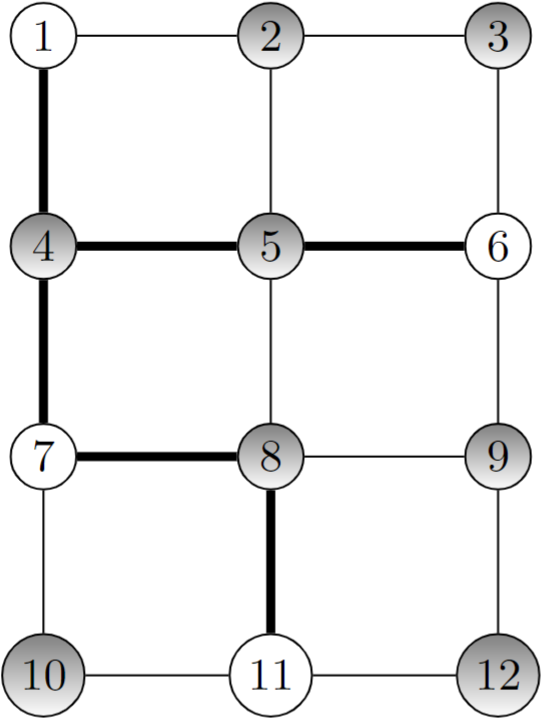
\includegraphics[width=.2\linewidth]{figure/steiner.png}
        \caption{a solution to steiner tree problem\cite{Nash_2020}}
    \end{figure}
\end{frame}
\begin{frame}
    \frametitle{generate tree}
    \begin{itemize}
        \item root $c$
        \item breadth first tree order 
        \item sub-tree rooted at terminal $c_i$
    \end{itemize}
\end{frame}
\begin{frame}
    \frametitle{sequence of row generations}
    \begin{itemize}
        \item start with last sub-tree
        \item sequence $R$: traverse the tree in reverse depth first order
        \item sequence $R^{'}=reverse(R-R[j])$
        \item sequence $R^{*}=R+R^{'}-R_{S}$
    \end{itemize}
\end{frame}

\subsection{algorithm}
\begin{frame}
    \frametitle{work flow}
    \begin{itemize}
        \item start with column $i=1$
        \item judge $(i,i)=0?$
        \item find steiner tree
        \item perform row operations and compute resulting matrix
        \item repeat 2-5
        \item transpose
    \end{itemize}
\end{frame}

\subsection{result}
\begin{frame}
    \frametitle{result for CNOT}
    \begin{figure}
        \centering
        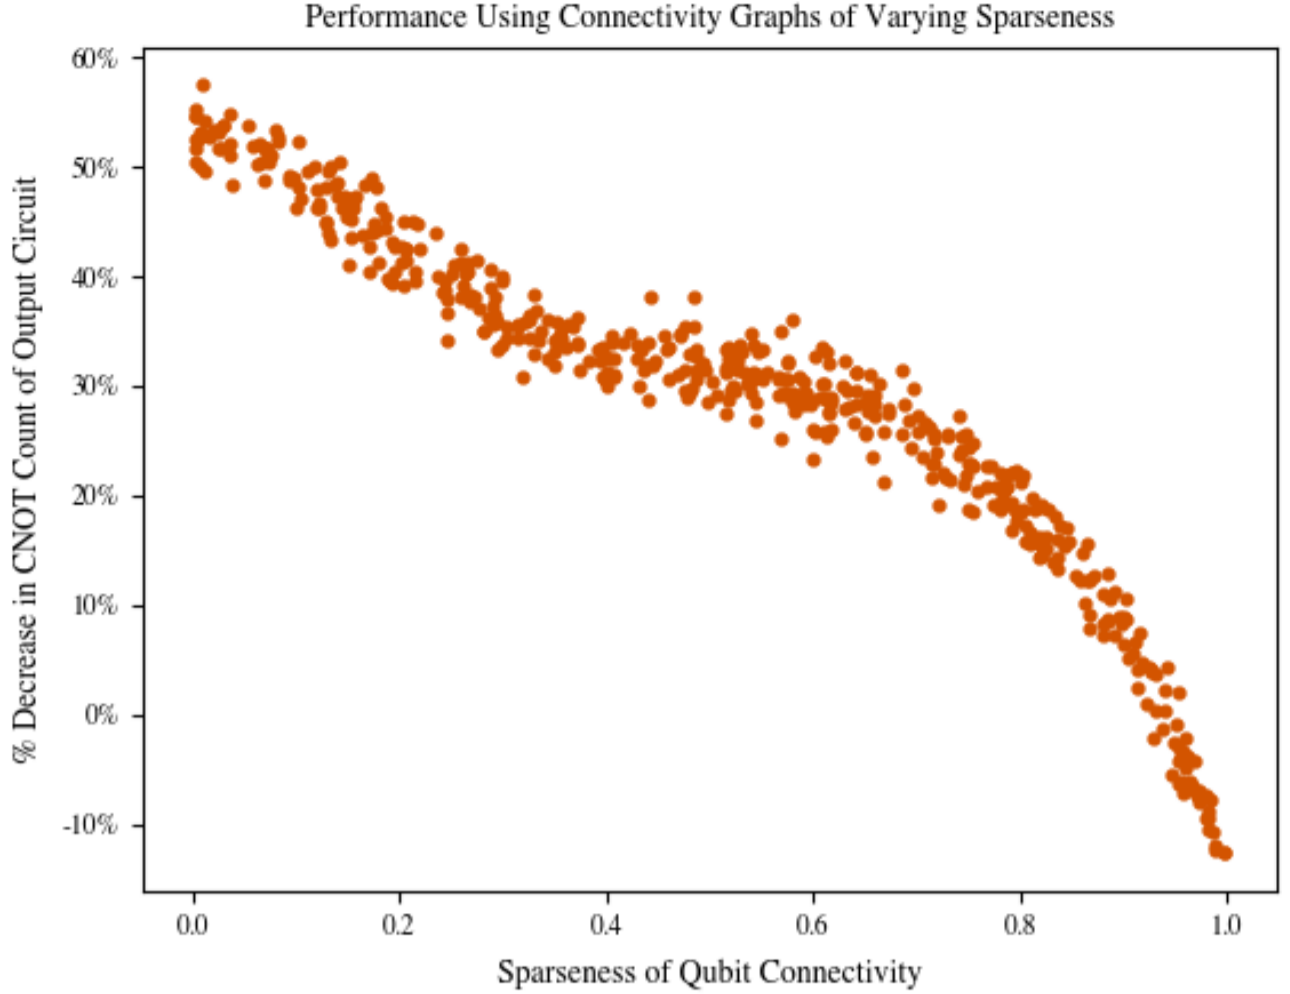
\includegraphics[width=.6\linewidth]{figure/CNOT-result.png}
        \caption{result for the synthesis of CNOT circuits on 20 qubits}
    \end{figure}
\end{frame}